\pdfoutput=1
\pdfcompresslevel=9
\pdfinfo
{
    /Author ()
    /Title ()
    /Subject ()
    /Keywords ()
}
%\documentclass[a4paper,onecolumn,twoside,12pt]{mwrep}
\documentclass[a4paper,openany,onecolumn,twoside,12pt]{book}
%\usepackage{times}
\usepackage[utf8x]{inputenc}
\usepackage[T1]{fontenc}
%\usepackage{wraptable}
\usepackage{amssymb}
\usepackage{setspace}
\usepackage{graphicx}
\usepackage{hyperref}
\usepackage{amsfonts}
\usepackage{amsmath}
\usepackage{amsthm}
\usepackage{float}
\usepackage{wrapfig}
\usepackage[nottoc]{tocbibind}
%\usepackage{algorithm}
%\usepackage[ruled]{algorithm2e}
\usepackage[ruled]{algorithm2e}
\usepackage{algpseudocode}
\usepackage{mathtools}
\usepackage{lipsum}
\usepackage{indentfirst}
\usepackage{listings}
\usepackage{algcompatible}
%\usepackage{subcaption}
\usepackage[square,numbers]{natbib}
\usepackage{multicol}
\usepackage[pscoord]{eso-pic}
\usepackage{fancyhdr}
\usepackage{tabularx}
%\usepackage{rotating}
%\usepackage{adjustbox}
%\usepackage[graphicx]{realboxes}
\newcolumntype{L}{>{\centering\arraybackslash}m{3cm}}
\newcolumntype{K}{>{\centering\arraybackslash}m{5cm}}
\usepackage{chngcntr}
\counterwithout{table}{chapter}
\usepackage{subfig}
%\usepackage[margin=1in]{geometry}
\usepackage{chngcntr}\counterwithout{figure}{chapter}
\usepackage[polish]{babel}
\fancypagestyle{plain}{%
  \fancyhf{}%
  \fancyfoot{}
  \renewcommand{\headrulewidth}{0pt}%
  \fancyhf[leh,roh]{\thepage}%
}

\hyphenpenalty=10000 % nie dziel wyrazów zbyt często
\clubpenalty=10000 % kara za sierotki
\widowpenalty=10000 % nie pozostawiaj wdów
\brokenpenalty=10000 % nie dziel wyrazów między stronami
\exhyphenpenalty=999999 % nie dziel słów z myślnikiem
\righthyphenmin=3 % dziel minimum 3 litery

\tolerance=4500
\pretolerance=250
\hfuzz=1.5pt
\hbadness=1450

\sloppy % umacnia pozycję prawego marginesu


%algo
\newenvironment{algorytm}[1][htb]
  {\renewcommand{\algorithmcfname}{Algorytm}% Update algorithm name
   \begin{algorithm}[#1]%
  }{\end{algorithm}}
 
  \newenvironment{eksperyment}[1][htb]
  {\renewcommand{\algorithmcfname}{Eksperyment}% Update algorithm name
   \begin{algorithm}[#1]%
  }{\end{algorithm}}
 
    \newenvironment{gra}[1][htb]
  {\renewcommand{\algorithmcfname}{Gra}% Update algorithm name
   \begin{algorithm}[#1]%
  }{\end{algorithm}}

\newenvironment{protokol}[1][htb]
    {\renewcommand{\algorithmcfname}{Protokół}
    \SetKwProg{zal}{Założenia}{}{}
    \SetKwProg{rola}{Rola}{}{}
    \SetKwProg{przeb}{Przebieg}{}{}
    \begin{algorithm}[#1]
   
    }{\end{algorithm}}

\newcommand{\matrices}[2]{\mathcal{M}_{#1 \times #2}[\GF(2^8)]}
\newcommand{\GF}{\mathrm{GF}}
\newcommand{\had}{\mathrm{had}}
\newcommand{\vdm}{\mathrm{vdm}}
\newcommand{\compository}{\mathop{\bigcirc}\displaylimits}
\newcommand{\gf}[1]{\textsf{`#1'}}
\setlength{\textwidth}{\paperwidth}
\addtolength{\textwidth}{-5cm}
\setlength{\textheight}{\paperheight}
\addtolength{\textheight}{-5cm}
\setlength{\oddsidemargin}{5cm}
\setlength{\evensidemargin}{0cm}
\topmargin -1.25cm
\footskip 1.4cm

\linespread{1.3}

\newtheorem{definition}{Definicja}

\newcommand{\placetextbox}[3]{% \placetextbox{<horizontal pos>}{<vertical pos>}{<stuff>}
  \setbox0=\hbox{#3}% Put <stuff> in a box
  \AddToShipoutPictureFG*{% Add <stuff> to current page foreground
    \put(\LenToUnit{#1\paperwidth},\LenToUnit{#2\paperheight}){\vtop{{\null}\makebox[0pt][c]{#3}}}%
  }%
}%

\usepackage{geometry}
\geometry{inner=3cm,outer=2.5cm}

%\input{algorytmy.tex}

\begin{document}
\pagenumbering{arabic}
%\pagenumbering{roman}

\begin{titlepage}
	\begin{center}
	\fontsize{28pt}{34pt}\selectfont
	WOJSKOWA AKADEMIA TECHNICZNA \\
	\fontseries{b}\fontsize{14pt}{20pt}\selectfont
	im. Jarosława Dąbrowskiego
	\vspace*{1.0\baselineskip}
	
	\fontseries{b}\fontsize{24pt}{20pt}\selectfont
	Wydział Cybernetyki
	
	\begin{figure}[!ht]
	    \centering
	    
\includegraphics{rysunki/logo_wat.png}
	\end{figure}
	

	%\vspace*{1\baselineskip}
	\fontseries{m}\fontsize{32pt}{20pt}\selectfont
	PRACA DYPLOMOWA \\
	\fontseries{m}\fontsize{20pt}{20pt}\selectfont
	Studia stacjonarne II$^\circ$\\
	\vspace*{1.15\baselineskip}
	%\fontsize{20pt}{15pt}\selectfont
	%sierż. pchor. Damian Krata\\
	%\vspace*{1.15\baselineskip}
	\fontseries{b}\fontsize{15pt}{18pt}\selectfont
	Analiza możliwości sprzętowej implementacji szyfru blokowego opartego o algorytm Anubis w sposób uodparniający na ataki kanałem bocznym \\
	\end{center}

	%\vspace*{2\baselineskip}
	%\put(0,0){\mbox{Autor \newline sierż. pchor. Damian Krata}}
	\placetextbox{0.25}{0.25}{Autor}
	\placetextbox{0.25}{0.23}{sierż. pchor. Damian Krata}
	
	\placetextbox{0.75}{0.25}{Promotor}
	\placetextbox{0.75}{0.23}{kpt. dr inż. Michał Wroński}
	
	
	%\begin{flushright}
	%\fontseries{m}\fontsize{13pt}{10pt}\selectfont
%	Promotor\\
	%dr inż. Piotr Bora\\
	%\end{flushright}
    %\baselineskip=16pt
	%\vspace*{7\baselineskip}
	%\vfill
	%\begin{center}
	%Warszawa 2017
	%\end{center}
	\placetextbox{0.5}{0.15}{Warszawa 2019}
\end{titlepage}

\setcounter{page}{2}

\Large
\vspace*{4\baselineskip}
\textbf{OŚWIADCZENIE}

\vspace*{0.8\baselineskip}
„Wyrażam zgodę na udostępnianie mojej pracy przez Archiwum  WAT”
\vspace*{0.4\baselineskip}
\placetextbox{0.3}{0.55}{\Large Dnia ..........................}
\placetextbox{0.7}{0.55}{\Large ..........................}
\placetextbox{0.7}{0.53}{ (podpis)}

\placetextbox{0.65}{0.45}{\Large Pracę przyjąłem}
\placetextbox{0.65}{0.40}{\Large promotor pracy}
\placetextbox{0.65}{0.37}{\Large kpt. dr inż. Michał Wroński}
\normalsize
\clearpage

\setcounter{page}{5}
\tableofcontents

\phantomsection
\chapter*{Wstęp}
\addcontentsline{toc}{chapter}{Wstęp}


\chapter{Algorytmy blokowe}

\section{Szyfry blokowe}
\textbf{Szyfr blokowy} jest funkcją, która odwzorowuje \textit{n-bitowy} blok tekstu jawnego na \textit{n-bitowy} blok szyfrogramu ($n$ nazywamy długością bloku). Może on być rozpatrywany jako prosty szyfr podstawieniowy o dużym rozmiarze znaku. Funkcję parametryzuje $k$-bitowy klucz $K$ przyjmujący wartości z podzbioru $\kappa$ (przestrzeń kluczy) zbiory wszystkich k-bitowych wektorów $V_k$. Zazwyczaj przyjmuje się, że klucz jest wybierany losowo. Stosowanie bloków tekstu jawnego i szyfrogramu o tej samej długości umożliwia uniknięcie rozrostu danych. Aby można było jednoznacznie odszyfrować dane, funkcja szyfrująca musi być typu jeden-do-jednego (tj. odwracalna). Dla $n$-bitowych bloków tekstu jawnego i szyfrogramu oraz ustalonego klucza funkcja szyfrująca jest bijekcją, definiującą permutację $n$-bitowych wektorów. Każdy klucz potencjalnie określa inną bijekcję. Liczba kluczy wynosi $|\kappa|$, a efektywna długość klucza $lg|\kappa|$. Odpowiada to długości klucza, jeśli wszystkie $k$-bitowe wektory są prawidłowymi kluczami ($\kappa=V_k$). Jeśli klucze są jednakowo prawdopodobne i każdy określa inną bijekcję, entropia przestrzeni kluczy również wynosi $lg|\kappa|$.

W symetrycznych algorytmach kryptograficznych do szyfrowania i deszyfrowania wykorzystywany jest ten sam klucz $K$. Konieczność ochrony tego klucza powoduje, ze algorytmy symetryczne określa się także jako algorytmy z \textit{tajnym} kluczem. Współcześnie istnieją dwie główne metody konstruowania szyfrów symetrycznych, które ze względu na rodzaj operacji, które są wykonywane w trakcie deszyfrowania i szyfrowania można podzielić na:
\begin{itemize}
\item algorytmy zbudowane na podstawie sieci Feistela (Lucifer, DES)
\item algorytmy zbudowane na podstawie sieci podstawieniowo - przestawieniowej (ang. \textit{substitution - permutation network} np. AES)
\end{itemize}

\begin{figure}[H]
  \centering
  \subfloat[Sieć Feistela. Źródło \cite{Feistel}.]{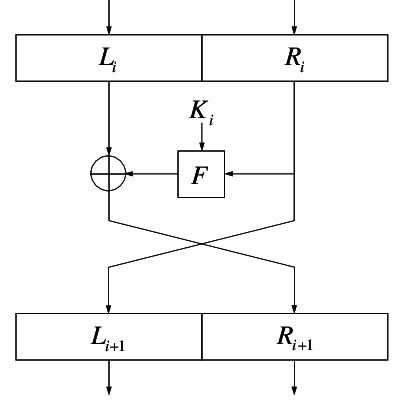
\includegraphics[width=0.5\textwidth]{rysunki/Blokowe/feistel2.png}}
  \hfill
  \subfloat[Sieć SP. Źródło \cite{SP}.]{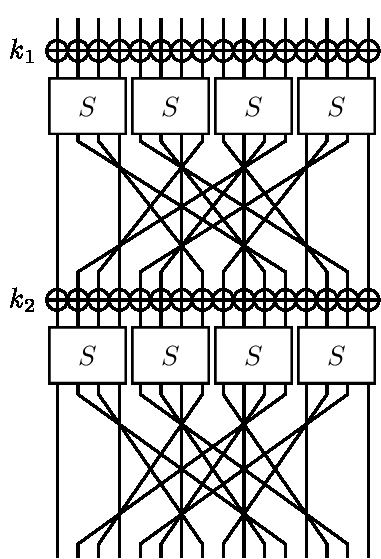
\includegraphics[width=0.5\textwidth]{rysunki/Blokowe/spnetwork2.png}}
  \caption{Porównanie dwóch sposobów budowy szyfrów blokowych}
  \label{fig:siec_feistela_sp}
\end{figure}

Ważnym elementem każdego szyfru symetrycznego jest sposób rozszerzania klucza głównego $K$ (ang. \textit{key schedule}). Pozwala on na zwiększenie długości klucza kryptograficznego zastosowanego w algorytmie, aby każda runda posiadała swój własny klucz zwany także kluczem rundy $K_r$ (ang. \textit{round key}). W większości systemów kryptograficznych, schemat generacji kluczy rund wykorzystuje takie same transformacje jak procedury szyfrowania/deszyfrowania.\footnote{Podrozdział na podstawie \cite{kryptografia_stosowana}.}

\section{Anubis}
Anubis jest 128 bitowym, iteracyjnym szyfrem blokowym z kluczami różnej długości. Pomimo tego, że nie jest on zbudowany w oparciu o sieć Feistela, jego struktura pozwala na wykonanie deszyfrowania, bez konieczności zmiany logiki modułów wykonujących przekształcenia. Jedyną różnicą pomiędzy szyfrowaniem a deszyfrowaniem, jest zmiana w kolejności wyboru klucza rundy uzgodnionego za pomocą schematu rozszerzania klucza. Powyższą właściwość osiągnięto dzięki zastosowaniu tzw. inwolucji, czyli operacji samo-odwrotnych. Zastosowanie tych operacji pozwala na zmniejszenie zajętości układów realizujących szyfrowanie i deszyfrowanie. 

Szyfr Anubis został zaprojektowany zgodnie ze Strategią Szerokiej Ścieżki (ang. \textbf{\textit{Wide Trail Strategy}}). W strategii tej, runda algorytmu złożona jest z różnych odwracalnych transformacji, które posiadają swoje funkcjonalności i mają określone wymagania. Liniowe warstwy dyfuzji zapewniają, że już po kilku rundach, bity wyjściowe zależą od wszystkich bitów wejściowych. Warstwy nieliniowe z kolei zapewniają powyższej zależności złożoną naturę, uniemożliwiającą wyprowadzenie zależności, rozwiązywalnych przy pomocy dostępnych narzędzi matematycznych. Operacja dodania klucza rundy pozwala na wprowadzenie dodatkowego materiału oraz uzależnia potok obliczeń od konkretnych danych wejściowych. 

Anubis jest inwolucyjnym szyfrem blokowym działającym na 128 bitowej macierzy stanu. Wykorzystuje on klucz o długości $32N$-bitów, gdzie ($4 \leqslant N\leqslant 10$) i składa się z kilku przekształceń macierzy stanu zależnych od klucza rundy.

Operacje wykonywane są w ciele $\GF(2^8)$ reprezentowanym jako $\GF(2)[x]/p(x)$, gdzie $p(x) = x^8 + x^4 + x^3 + x^2 + 1$ jest wielomianem nierozkładalnym. Wielomian ten został tak dobrany, aby $g(x) = x$ było generatorem $\GF(2^8) \setminus \{0\}$.

Element $u = u_7 x^7 + u_6 x^6 + u_5 x^5 + u_4 x^4 + u_3 x^3 + u_2 x^2 + u_1 x + u_0$ ciała $\GF(2^8)$ gdzie $u_i \in \GF(2)$ dla każdego $i = 0, \dots, 7$, będzie oznaczony przez wartość numeryczną $u_7
\cdot 2^7 + u_6 \cdot 2^6 + u_5 \cdot 2^5 + u_4 \cdot 2^4 + u_3
\cdot 2^3 + u_2 \cdot 2^2 + u_1 \cdot 2 + u_0$, zapisaną w postaci hexadecymalnej. Dla przykładu $u = x^4 + x + 1$ odpowiada ${13_{hex}}$. Wielomianowi redukującemu $p(x)$ odpowiada ${11d_{hex}}$


\subsection{Dane wejściowe i wyjściowe}
Stan szyfru jest definiowany za pomocą macierzy $\matrices{4}{4}$, podczas gdy klucz za pomocą macierzy $\matrices{N}{4}$. W związku z tym, 128-bitowe bloki danych oraz $32N$-bitowe bloki klucza są mapowane w formie macierzy. Działanie to wyraża się poprzez funkcję 
$\mu: \GF(2^8)^{4N} \rightarrow \matrices{N}{4}$ i jej odwrotność:
\[
\mu(a) = b \,\Leftrightarrow\, b_{ij} = a_{4i + j}, \; 0
\leqslant i \leqslant N-1, \; 0 \leqslant j \leqslant 3.
\]

\subsection{Warstwa nieliniowa $\gamma$}
Funkcja $\gamma: \matrices{N}{4} \rightarrow \matrices{N}{4}$,
$4 \leqslant N \leqslant 10$, składa się z równolegle działających skrzynek podstawieniowych $S: \GF(2^8) \rightarrow
\GF(2^8), \, x \mapsto S[x]$, które realizują podstawienie każego bajtu z osobna:
\[
\gamma(a) = b \,\Leftrightarrow\, b_{ij} = S[a_{ij}], \; 0
\leqslant i \leqslant N-1, \; 0 \leqslant j \leqslant 3.
\]
Sbox został wybrany pseudo - losowo tak, aby zapewnić warunek:
$S[S[x]] = x$ dla każdego $x \in \GF(2^8)$.

\subsection{Transpozycja $\tau$}
Mapowanie $\tau: \matrices{4}{4} \rightarrow \matrices{4}{4}$
transponuje elementy macierzy stanu:
\[
\tau(a) = b \,\Leftrightarrow\, b = a^t \,\Leftrightarrow\, b_{ij}
= a_{ji}, \; 0 \leqslant i, j \leqslant 3.
\]
Transpozycja jest inwolucją.

\subsection{Warstwa dyfuzji $\theta$}

W algorytmie Anubis, rozproszenie danych realizowane jest przy pomocy przekształcenia $\theta: \matrices{N}{4} \rightarrow
\matrices{N}{4}$, $4 \leqslant N \leqslant 10$. Jest to liniowe przypisanie wartości odpowiadających działaniu:
\[
\theta(a) = b \,\Leftrightarrow\, b = a \cdot H,
\]
gdzie $H = \had(\gf{01}, \gf{02}, \gf{04},\gf{06})$, tzn.
\[
H = \left[\begin{array}{cccc} %
\gf{01} & \gf{02} & \gf{04} & \gf{06}\\
\gf{02} & \gf{01} & \gf{06} & \gf{04}\\
\gf{04} & \gf{06} & \gf{01} & \gf{02}\\
\gf{06} & \gf{04} & \gf{02} & \gf{01}
\end{array}\right]
\]

\subsection{Dodanie klucza $\sigma[k]$}

Liniowe dodanie klucza rundy $\sigma[k]: \matrices{N}{4} \rightarrow
\matrices{N}{4}$, $4 \leqslant N \leqslant 10$ sprowadza się do wykonania operacji $\oplus$ na aktualnie przetwarzanej macierzy stanu i macierzy klucza $k \in \matrices{N}{4}$:
\[
\sigma[k](a) = b \,\Leftrightarrow\, b_{ij} = a_{ij} \oplus
k_{ij}, \; 0 \leqslant i \leqslant N-1, \; 0 \leqslant j
\leqslant 3.
\]

\subsection{Cykliczna permutacja $\pi$}

Permutacja  $\pi: \matrices{N}{4} \rightarrow \matrices{N}{4}$,
$4 \leqslant N \leqslant 10$, cyklicznie przesuwa każdą kolumnę oddzielnie do dołu, w ten sposób, że kolumna $j$ jest przesuwana o $j$ pozycji:

\[
\pi(a) = b \,\Leftrightarrow\, b_{ij} = a_{(i-j) \bmod N, j}, \;
0 \leqslant i \leqslant N-1, \; 0 \leqslant j \leqslant 3.
\]

\subsection{Ekstrakcja klucza $\omega$}

Przekształcenie ekstrakcji klucza jest funkcją $\omega: \matrices{N}{4} \rightarrow
\matrices{4}{4}$, $4 \leqslant N \leqslant 10$, sprowadza się do wykonania

\[
\omega(a) = b \,\Leftrightarrow\, b = V \cdot a,
\]
gdzie $V = \vdm_N(\gf{01}, \gf{02},\gf{06},\gf{08})$, tzn.

\[
V = \left[\begin{array}{lllcl} %
\gf{01} & \gf{01} & \gf{01}^{} & \dots & \gf{01}^{}\\
\gf{01} & \gf{02} & \gf{02}^2 & \dots & \gf{02}^{N-1}\\
\gf{01} & \gf{06} & \gf{06}^2 & \dots & \gf{06}^{N-1}\\
\gf{01} & \gf{08} & \gf{08}^2 & \dots & \gf{08}^{N-1}
\end{array}\right],
\]

\subsection{Stałe rundy $c^r$}
$r$-ta stała rundy ($r > 0$) jest macierzą $c^r \in
\matrices{N}{4}$, $4 \leqslant N \leqslant 10$, zdefiniowaną jako:
\[
\begin{array}{lcll}
c_{0j}^r & = & S[4(r - 1) + j], & 0 \leqslant j \leqslant 3,\\
c_{ij}^r & = & 0, & 1 \leqslant i < N, 0 \leqslant j \leqslant 3.
\end{array}
\]

\subsection{Schemat klucza}

Schemat klucza (ang. \textit{key schedule}) rozszerza klucz $K \in \GF(2^8)^{4N}$, $4
\leqslant N \leqslant 10$, na klucze rund $K^0,\dots, K^R$, gdzie $K^r \in \matrices{4}{4}$:
\begin{eqnarray*}
\kappa^0 & = & \mu(K),\\
\kappa^r & = & (\sigma[c^r] \circ \theta
\circ \pi \circ \gamma)(\kappa^{r-1}), \;\; r > 0,\\
K^r & = & (\tau \circ \omega \circ \gamma)(\kappa^r), \;\; 0
\leqslant r \leqslant R;
\end{eqnarray*}

Przekształcenie $\psi[c^r] \equiv \sigma[c^r] \circ \theta
\circ \pi \circ \gamma$ nazywane jest funkcją rozwoju $r$-tego klucza rundy podczas gdy $\phi \equiv \tau \circ \omega \circ \gamma$ nazywane jest funkcją wyboru klucza. W ogólności w fazie obliczeń, wyznaczanie klucza rundy sprowadza się do wykonania funkcji $\phi$ na kluczu poddawanym obliczeniom za pomocą funkcji $\psi$.


\subsection{Matematyczny opis algorytmu}
Dla klucza $K \in \GF(2^8)^{4N}$, Anubis może być zdefiniowany jako przekształcenie $\textsc{Anubis}[K]: \GF(2^8)^{16} \rightarrow \GF(2^8)^{16}$ zadane przez
\[
\textsc{Anubis}[K] \equiv \mu^{-1} \circ \alpha_R[K^0, \dots, K^R] \circ \mu,
\]
gdzie

\[
\alpha_R[K^0, \dots, K^R] = \sigma[K^R] \circ \tau \circ \gamma
\circ \left(\compository^{r=R-1}_1{\sigma[K^r] \circ \theta \circ
\tau \circ \gamma}\right) \circ \sigma[K^0].
\]

Standardowa liczba rund dla algorytmu $R$ określona jest jako $R = 8 + N$ dla $32N$-bitowego klucza, $4 \leqslant N \leqslant 10$. Przekształcenie $\rho[K^r] \equiv \sigma[K^r] \circ \theta \circ \tau
\circ \gamma$ nazywane jest \textit{funkcją rundy}, natomiast $\rho'[K^R] \equiv \sigma[K^r]
\circ \tau \circ \gamma$ pozbawione $\theta$ określane jest jako \textit{funkcja ostatniej rundy}.

\subsection{K - bezpieczeństwo}
\begin{definition}[\cite{joan}]
Szyfr blokowy jest K - bezpieczny, jeśli wszystkie możliwe strategie ataku na niego, mają ten sam oczekiwany współczynnik wymagań pamięciowych i obliczeniowych, jak większość szyfrów blokowych z takim samym rozmiarem klucza.Powyższe odnosi się do wszystkich znanych ataków (ze znanym tekstem jawnym, szyfrogramem, atakiem adaptacyjnym itp.).
\end{definition}

K - bezpieczeństwo jest bardzo silnym pojęciem. System kryptograficzny nie może zostać uznany za K - bezpieczny jeśli wystąpi co najmniej jeden z następujących przypadków:
\begin{itemize}
    \item istnieje atak szybszy niż brutalne przeszukanie,
    \item występuje właściwość symetrii w przekształceniach,
    \item istnieje klasa kluczy słabych, których istnienie nie jest pomijalne,
    \item możliwy jest atak z kluczami zależnymi.\footnote{Podrozdział na podstawie \cite{anubis_dokumentacja}.}
\end{itemize}



\section{Advanced Encryption Standard - AES}

AES - zaawansowany standard szyfrowania, powstał jako nowy standard szyfrowania przyjęty przez NIST w 2001 roku. Miał za zadanie zastąpić algorytm DES (ang. \textit{Data Encryption Standard}). Oparty został na finaliście konkursu na AES - algorytmie Rijndael. AES jest szyfrem blokowym. W przeciwieństwie do poprzedniego standardu, DES'a działającego na zasadzie sieci Feistel'a, zbudowany jest w oparciu o sieć permutacyjno - podstawieniową (ang. \textit{SPN Network}). Na rundę algorytmu AES składają się cztery przekształcenia, które polegają na wykonywaniu działań realizowanych w ciele $GF(2^8)$:
\begin{enumerate}
	\item \textbf{\textit{AddRoundKey}} - przekształcenie polegające na dodaniu klucza rundy w każdej iteracji algorytmu,
	\item \textbf{\textit{MixColumns}} - przekształcenie kolumn macierzy stanu,
	\item \textbf{\textit{ShiftRows}} - przesunięcie cykliczne trzech ostatnich wierszy w macierzy stanu o określoną liczbę,
	\item \textbf{\textit{SubBytes}} - zamiana bajtów - operacja nieliniowa realizowana za pomocą skrzynki podstawieniowej.
\end{enumerate}

Algorytm wykonuje szyfrowanie bloków danych wielkości 128 - bitów za pomocą klucza K długości 128, 192 lub 256 bitów. W zależności od długości klucza, wersje algorytmu AES różnią się między sobą liczbą wykonywanych rund. 
\begin{itemize}
    \item 10 rund dla klucza 128 - bitowego,
    \item 12 rund dla klucza 192 - bitowego,
    \item 14 rund dla klucza 256 - bitowego,
\end{itemize}
W każdej rundzie, poza ostatnią, wykonywane są wszystkie przekształcenia przedstawione powyżej. Dla ostatniej rundy, schemat nie realizuje operacji MixColumns.

 Blok danych reprezentowany jest w algorytmie w postaci macierzy, składającej się z szesnastu 8-bitowych elementów, nazywanej \textit{Stanem $S$}. 

\begin{figure}[H]
    \centering
    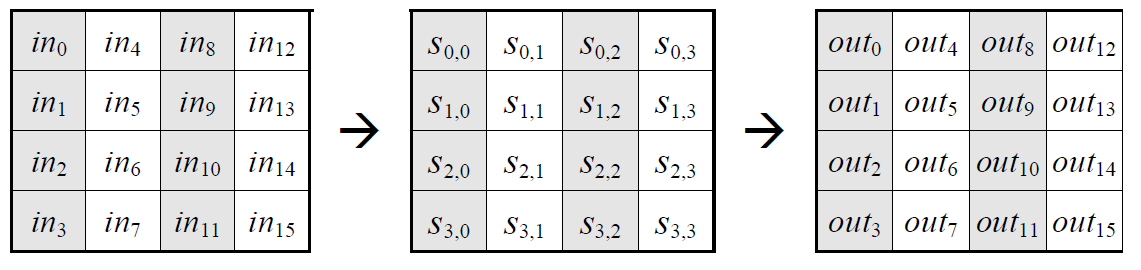
\includegraphics[width=\textwidth]{rysunki/AES_opis/state.PNG}
    \caption{Macierz stanu. Źródło \cite{fips_197}.}
    \label{fig:state_macierz}
\end{figure}

Wykonywanie dodawania $a(x) \oplus b(x)$ na dwóch elementach ciała $GF(2^8)$ sprowadza się do wykonywania operacji XOR dla odpowiadających współczynników $a(x)$ i $b(x)$. Sytuacja komplikuje się w przypadku obliczania iloczynu dwóch elementów. Wielomianem nierozkładalnym użytym w algorytmie AES jest:
\begin{center}
$p(x)=x^8+x^4+x^3+x+1$
\end{center}
Zatem wszystkie operacje realizowane są modulo ten wielomian.

W implementacjach, najczęściej wykorzystuje się fakt, że pomnożenie elementu w ciele $GF(2^8)$ sprowadza się do jego bitowego przesunięcia w lewo i wykonaniu operacji modulo z $11b_{hex}$ w przypadku, gdy najstarszy bit (skrajny lewy) był równy zero.

\subsection{AddRoundKey}
Przekształcenie AddRoundKey pozwala na wprowadzenie do algorytmu klucza rundy. Polega ona na wykonaniu dodawania modularnego. Klucz rundy powstaje z klucza głównego za pomocą algorytmu rozszerzania klucza i przedstawiany jest w postaci macierzy $4 \times 4$. Wynikowa macierz stanu ma postać:
\begin{center}
$S'=[s^{'}_{i,j}]_{4 \times 4}$ gdzie $s^{'}_{i,j}=s_{i,j} \oplus k_{i,j}$
\end{center}
Transformacja AddRoundKey przebiega w ten sam sposób w czasie szyfrowania i deszyfrowania.

\begin{figure}[H]
    \centering
    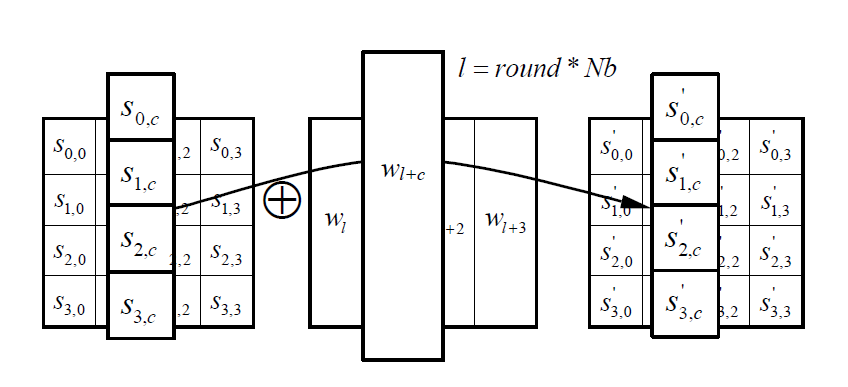
\includegraphics[width=0.8\textwidth]{rysunki/AES_opis/addroundkey.PNG}
    \caption{Przekształcenie AddRoundKey. Źródło \cite{fips_197}.}
    \label{fig:addroundkey}
\end{figure}

\subsection{MixColumns}
W przekształceniu MixColumns, cztery bajty każdej kolumny stanu są łączone za pomocą odwracalnej transformacji liniowej. Bajty te są następnie poddawane obliczeniom, które można zapisać w postaci macierzowej następująco:
\begin{center}
$S'=[W^{'}_{j}]_{1 \times 4}$ gdzie $W^{'}_{j}=
\begin{bmatrix} 
  s^{'}_{0,j} \\
  s^{'}_{1,j} \\
  s^{'}_{2,j} \\
  s^{'}_{3,j}
\end{bmatrix}
=
\begin{bmatrix} 
  02 & 03 & 01 & 01 \\
  01 & 02 & 03 & 01 \\
  01 & 01 & 02 & 03 \\
  03 & 01 & 01 & 02 
\end{bmatrix}
\begin{bmatrix} 
  s_{3,j} \\
  s_{2,j} \\
  s_{1,j} \\
  s_{0,j}
\end{bmatrix}
$
\end{center}

\begin{figure}[H]
    \centering
    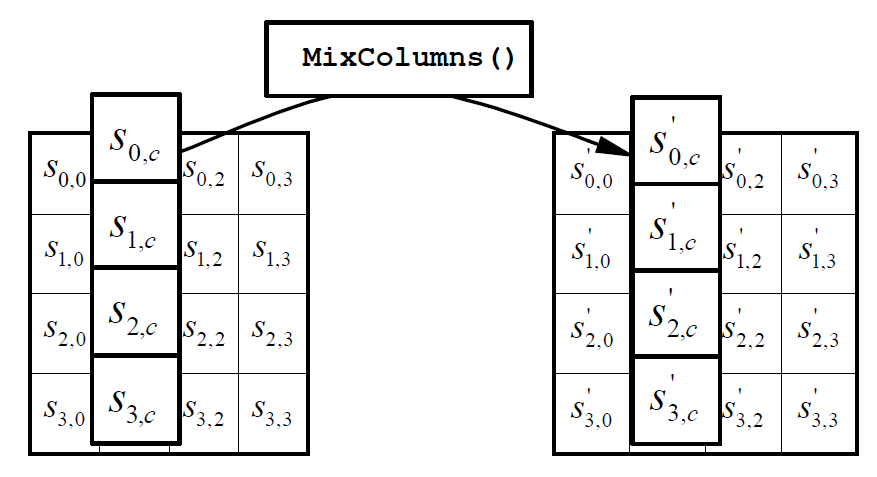
\includegraphics[width=0.7\textwidth]{rysunki/AES_opis/mixcolumns.PNG}
    \caption{Przekształcenie MixColumns. Źródło \cite{fips_197}.}
    \label{fig:mixcolumns}
\end{figure}

\subsection{ShiftRows}
Przekształcenie ShiftRows powoduje cykliczne przesunięcie wierszy macierzy stanu $S$ w lewo o różną liczbę pozycji bajtowych. Dla AES rotacje są następujące:
\begin{itemize}
	\item 1 wiersz macierzy - nie jest przesuwany,
	\item 2 wiersz macierzy - przesunięcie o 1 pozycję,
	\item 3 wiersz macierzy - przesunięcie o 2 pozycje,
	\item 4 wiersz macierzy - przesunięcie o 3 pozycje.
\end{itemize}

\begin{figure}[H]
    \centering
    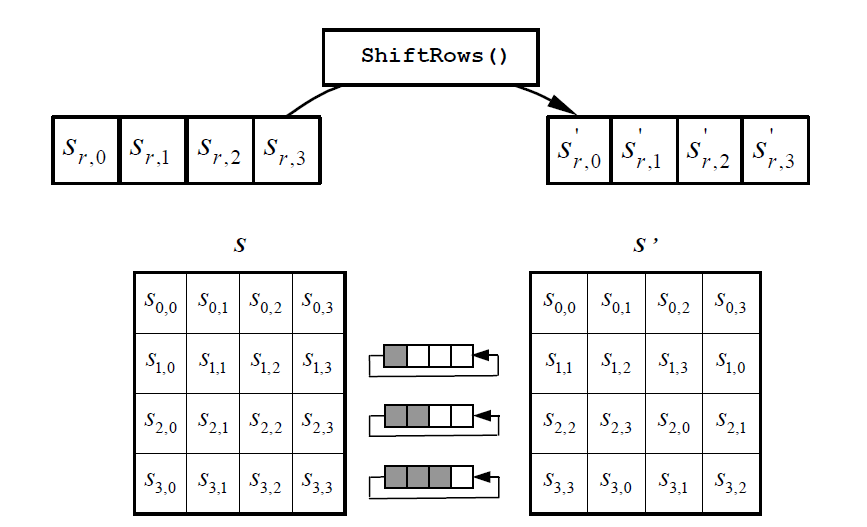
\includegraphics[width=0.7\textwidth]{rysunki/AES_opis/shiftrows.PNG}
    \caption{Przekształcenie ShiftRows. Źródło \cite{fips_197}.}
    \label{fig:shiftrows}
\end{figure}

Do deszyfracji używana jest podobna transformacja, z tą różnicą, że wiersze przesuwane są w prawo.

\subsection{SubBytes}

W przekształceniu SubBytes, każdy bajt macierzy stanu, jest zastępowany za pomocą 8-bitowej skrzynki podstawieniowej. Operacja ta jest nieliniowa, co znacząco poprawia właściwości algorytmu. Wykorzystany w algorytmie Sbox nie jest zwyczajną tablicą podstawień utworzoną empirycznie i przeanalizowaną. Wartości znajdujące się w niej mają swoje pochodzenie w działaniu obliczania odwrotności multiplikatywnej w ciele $GF(2^8)$. W celu uniknięcia ataków opierających się na właściwościach algebraicznych, postanowiono dołożyć do obliczania odwrotności przekształcenie afiniczne. Operacja SubBytes nie jest operacją samoodwrotną, co oznacza, że w celu deszyfracji należy zamienić kolejność wykonywania się poszczególnych jej składowych.

\begin{figure}[H]
    \centering
    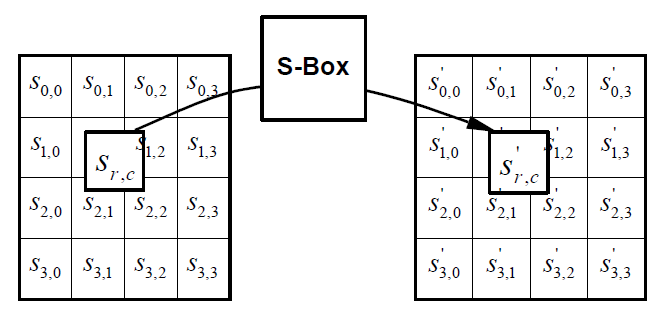
\includegraphics[width=0.7\textwidth]{rysunki/AES_opis/subbytes.PNG}
    \caption{Przekształcenie SubBytes. Źródło \cite{fips_197}.}
    \label{fig:subbytes}
\end{figure}
Przekształcenie afiniczne można sprowadzić do wykonania działań:
\begin{center}
$ s'_{i,j}=(F1\otimes s^{-1}_{i,j}\oplus 63) mod 101=
\begin{bmatrix} 
  1 & 1 & 1 & 1 & 0 & 0 & 0 & 1 \\
  1 & 1 & 1 & 0 & 0 & 0 & 1 & 1 \\
  1 & 1 & 0 & 0 & 0 & 1 & 1 & 1 \\
  1 & 0 & 0 & 0 & 1 & 1 & 1 & 1 \\
  0 & 0 & 0 & 1 & 1 & 1 & 1 & 1 \\
  0 & 0 & 1 & 1 & 1 & 1 & 1 & 0 \\        
  0 & 1 & 1 & 1 & 1 & 1 & 0 & 0 \\
  1 & 1 & 1 & 1 & 1 & 0 & 0 & 0 \\
\end{bmatrix}
\begin{bmatrix} 
  {s^{-1}_{i,j}}^{(7)} \\
  {s^{-1}_{i,j}}^{(7)} \\
  {s^{-1}_{i,j}}^{(7)} \\
  {s^{-1}_{i,j}}^{(7)} \\
  {s^{-1}_{i,j}}^{(7)} \\
  {s^{-1}_{i,j}}^{(7)} \\
  {s^{-1}_{i,j}}^{(7)} \\
  {s^{-1}_{i,j}}^{(7)}
\end{bmatrix}
\oplus
\begin{bmatrix} 
  0  \\
  1  \\
  1  \\
  0  \\
  0  \\
  0  \\        
  1  \\
  1  
\end{bmatrix}
$
\end{center}
Ze względu na dużą złożoność obliczeniową algorytmu wyznaczania odwrotności multiplikatywnej, zazwyczaj tablicuje się wartości. Niestety to rozwiązanie zwiększa wymagania pamięciowe.\footnote{Podrozdział na podstawie \cite{fips_197}.}
\newpage
\section{Porównanie Anubis i AES}

\begin{table}[!ht]
\centering
\begin{tabular}{ | L|| K| K |} 
\hline
 & AES & Anubis \\ 
\hline
\hline
Rozmiar bloku & 128 & 128 \\ 
\hline
Rozmiar klucza & 128, 192, 256 & 128, 160, 192, 224, 256, 288, 320 \\ 
\hline
Liczba rund & 10, 12, 14 & 12, 13, 14, 15, 16, 17, 18 \\ 
\hline
Schemat tworzenia kluczy & algorytm dedykowany \textit{a priori} & funkcje rozwijania i wyboru klucza \\ 
\hline
Wielomian redukujący $GF(2^8)$ & $x^8+x^4+x^3+x+1$ ($0x11B$) & $x^8+x^4+x^3+x^2+1$ ($0x11D$)\\ 
\hline
Pochodzenie Sbox'a & odwrotność w ciele $GF(2^8)$ i przekształcenie afiniczne & losowo wybrana inwolucja\\ 
\hline
Pochodzenie stałych rundy & wielomiany $x^i$ nad $GF(2^8)$ & kolejne wejścia do Sbox'a\\ 
\hline
\end{tabular}
\caption{\label{tab:comparison}Porównanie dwóch szyfrów blokowych. Źródło  \cite{strona_anubis}.}
\end{table}    



%\input{.tex}

%\input{implementacja.tex}

%\phantomsection
\chapter*{Podsumowanie}
\addcontentsline{toc}{chapter}{Podsumowanie}



\bibliography{bibliografia}
\nocite{*}
\bibliographystyle{plainnat}
\listoffigures
%\nocite{*}
%\bibliographystyle{plainnat}

\end{document}

% ex: set tabstop=4 shiftwidth=4 softtabstop=4 noexpandtab fileformat=unix filetype=tex spelllang=pl,en spell:

